
\begin{figure*}[t]
    \centering
    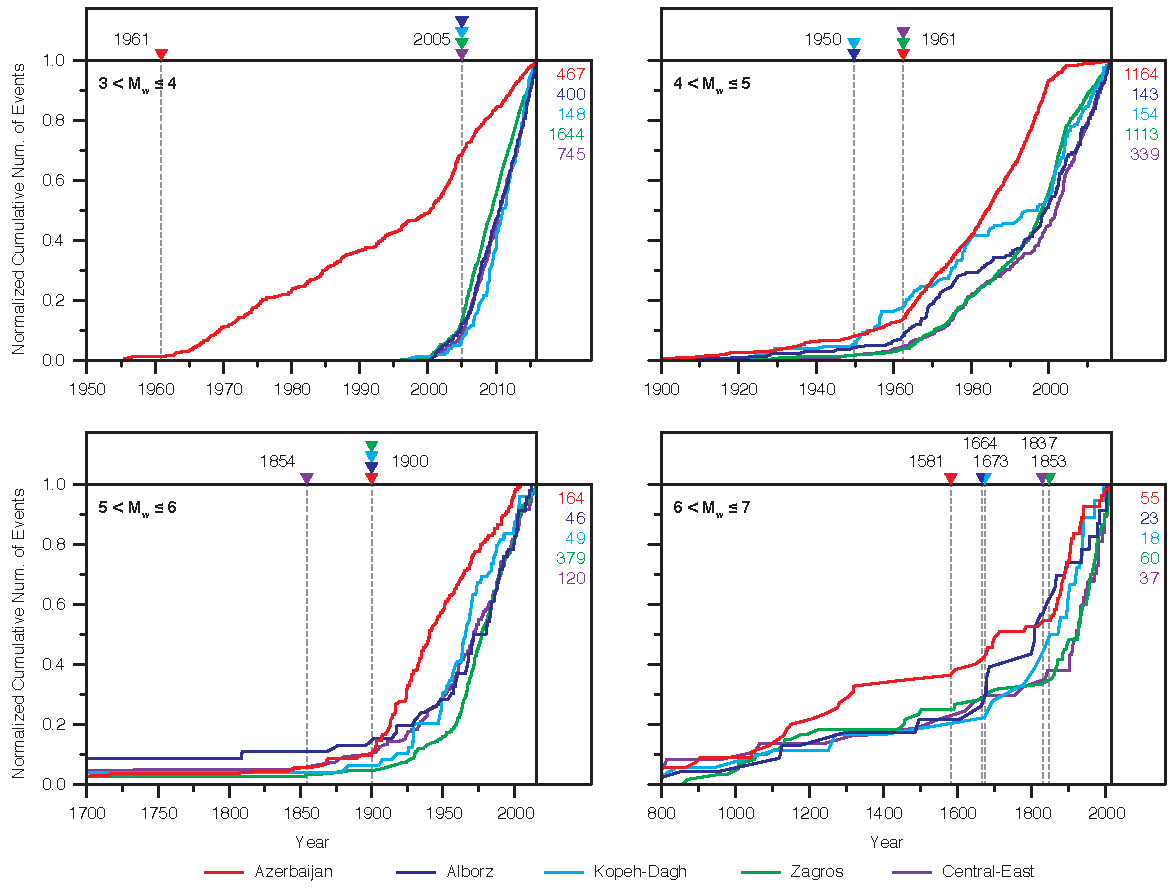
\includegraphics[width=0.8\textwidth]{figures/pdf/figure-05.pdf} 
    \caption{Normalized cumulative number of events and completeness year thresholds for each of the seismic zones considered within the region of interest, and for magnitude intervals of $\Delta M = 1$ between $M_w$ 3 and 7. The year thresholds are indicated by a triangle mark at the top and the vertical dashed lines in the background. Normalization values for each curve are indicated on the right margins and distinguished by color as indicated in the legend.}
    \label{fig:completeness}
\end{figure*}

\subsection{Completeness}

An important aspect of seismic catalogs is their completeness. This characteristic is measured in terms of the start-year of completeness and the completeness magnitude, which are both parameters that are later used in the seismic analysis process. The start-year of completeness is the point in time at which catalog data exhibit a steady rate of event occurrence or record accumulation for a certain magnitude range \myrevision{which in this study we use these values in estimating $a-values$ of smoothed seismic hazard}, and the completeness magnitude ($M_c$) is the magnitude above which the seismic catalog of a region can be considered complete within a certain time period. \myrevision{ We use $M_c$ for each catalog to compute the $b-value$ and $M_{max}$}

The start-year of completeness is commonly identified by inspection. A simple approach used by \citet{Frankel1995} and others is to select the year at which a plot of the cumulative number of events with respect to time becomes (or starts to resemble) a straight line. This is done for different magnitude ranges. Following this approach, we determined the year of completeness for magnitude ranges 3--4, 4--5, 5--6 and 6--7. Our choices are illustrated in Fig.~\ref{fig:completeness}, where we show the normalized cumulative number of events with time for each of the seismic zones and magnitude ranges, and indicate our selection of the year of completeness in each case. The values shown in this figure and those corresponding to the uniform model of the entire region of interest are summarized in Table \ref{tab:completeness}. For events $M_w>7$, in which case there are insufficient data to determine a proper threshold, we assumed the catalog to be complete from the earliest time at which there is record of large magnitude earthquakes. 

Determining the completeness magnitude $M_c$, on the other hand, is often determined using simple numerical analysis in combination with data inspection. Two common approaches are maximum curvature and the goodness-of-fit test methods. The maximum curvature method, or MAXC for simplicity, is widely used because as it has been implemented in the ZMAP software package for seismic hazard analysis developed by \citet{Wiemer2001}. \citet{Zare2014}, for instance, used this software to identify $M_c$ values for the different regions of the Middle East. We use the goodness-of-fit test method introduced by \citet{Wiemer2000}, and compute $M_c$ for different catalog-time intervals, namely 1800--1899, 1900--1999, 2000--2015, and for the complete regional catalogs.

We defined these year intervals based on the data magnitude-time distribution (see Fig.~\ref{fig:scatter}) and the idea of distinguishing between historical, early-instrumental, and modern-instrumental catalogs. Having augmented the original catalog with $M>3$ earthquakes beginning in 2000 also influenced our choice of the intervals because at this point the uniformity of the catalog is altered. Last, we also computed $M_c$ values for the complete regional catalogs, but in this case, in order to maintain uniformity throughout time, we only considered $M>4$ events. Fig.~\ref{fig:mc} illustrates the selection of $M_c$ for the case of the main three northern Iran seismic regions, and Table \ref{tab:completeness} presents the final selection of $M_c$ values for these and the other regions, including the uniform northern Iran model for the complete region of interest.

The values of $M_c$ for different time intervals and seismic regions are used to determine the seismicity Gutenberg-Richter parameters $b$ and $M_{\max}$ (see Section \ref{sec:params}), and the $M_c$ values for the complete regional catalogs and the start-years of completeness are used later for computing the hazard. Admittedly, the choice of the start-years is highly subjective. We should note then, that in the process of choosing the points indicated in the plots shown in Fig.~\ref{fig:completeness}, we considered additional contributing information such as the history of instrumentation. It is well known that the number of recorded earthquakes increased considerably after the first deployment of seismic instruments in the early 1900s, and later with the establishment of the Worldwide Standardized Seismograph Network in 1961. We compared our choices with the year thresholds reported by \citet{Zare2014}, which we found to be consistently earlier than our preferred years of completeness. In the end, our selection should lead to a slightly more conservative estimations of hazard. For the case of $M_c$, we compared our results with the values reported by \citet{Karimiparidari2013} and \citet{Khodaverdian_2016_BSSA} and found them to be in general good agreement, despite differences in the spatial definition of the seismic zones.

\begin{figure*}[t]
    \centering
    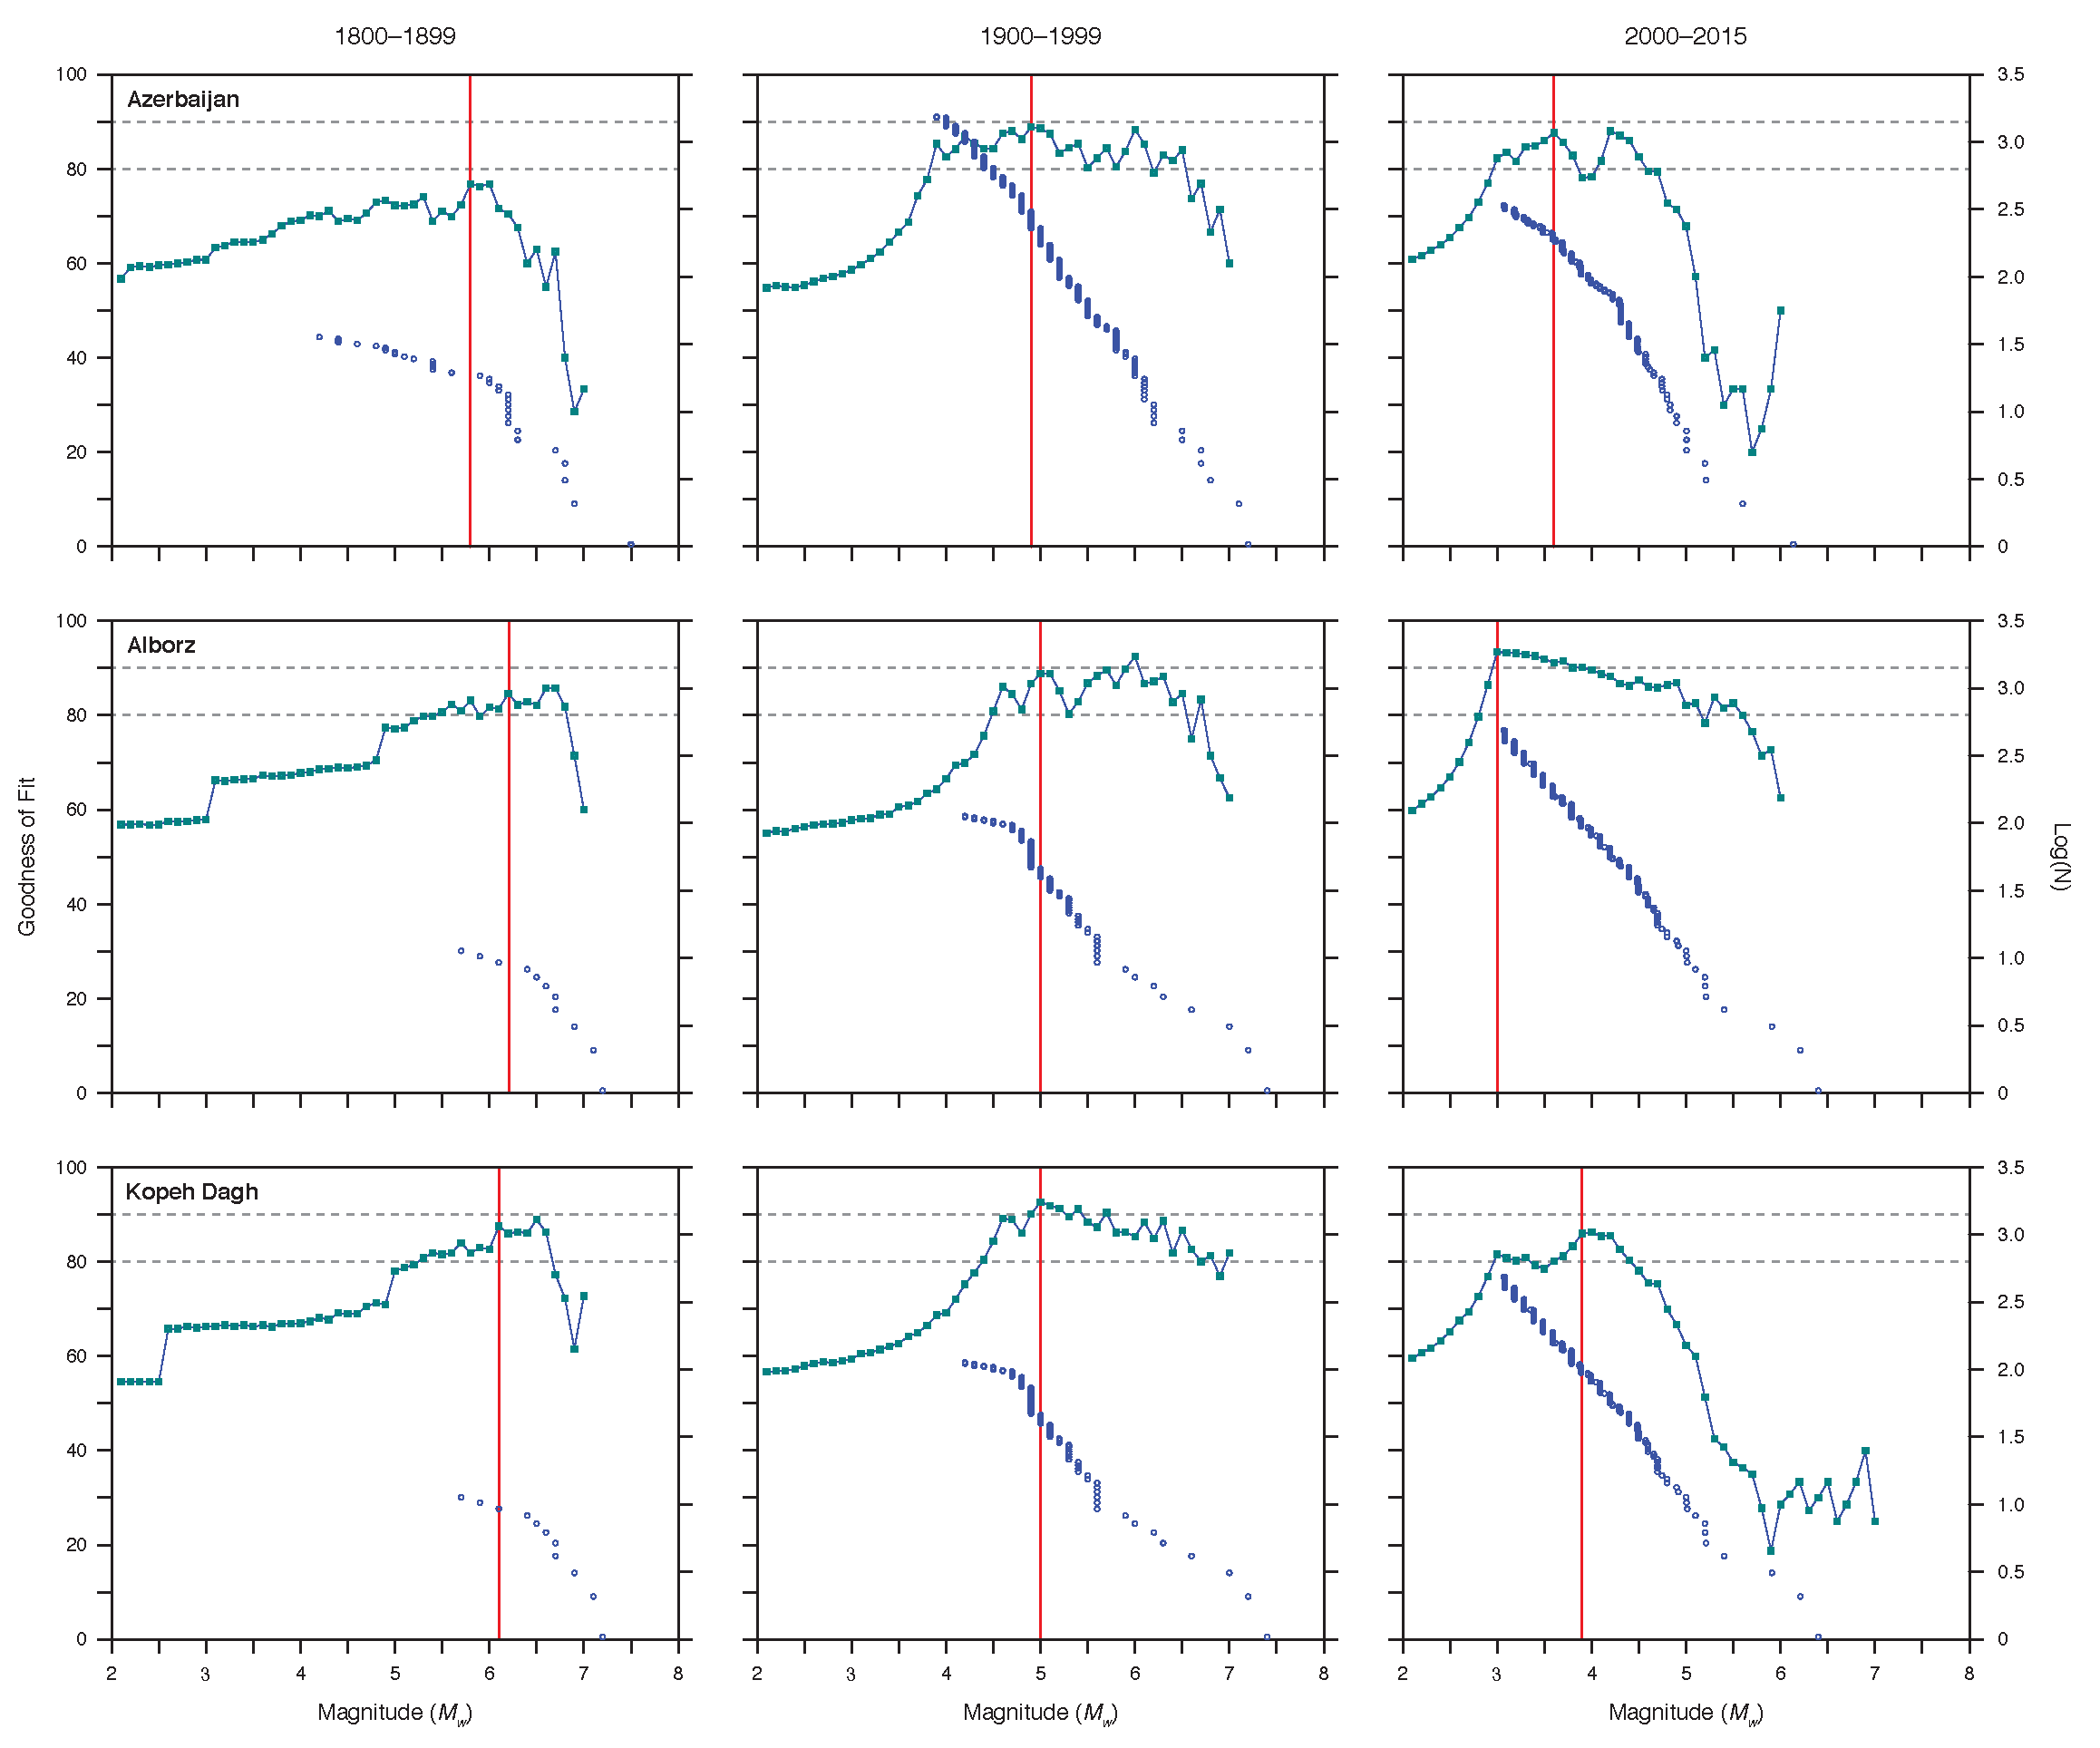
\includegraphics[width=\textwidth]{figures/pdf/figure-06.pdf} 
    \caption{Selection of completeness magnitude ($M_c$) values for the three main seismic regions in northern Iran. The blue squares indicate the computed goodness-of-fit test values and the green circles indicate the cumulative number of events. Both are shown as functions of the earthquake magnitude. The former is plotted in linear scale (left axes) and the latter is plotted in logarithmic scale (right axes). The horizontal dashed lines indicate desired thresholds for the goodness-of-fit values at 80 and 90 percent. The vertical red lines indicate the chosen $M_c$ values for each zone and catalog year interval.}
    \label{fig:mc}
\end{figure*}

\begin{table*}%[t]
    \centering
    \caption{Year thresholds and magnitude completeness for the seismic zones within the region of interest in this study. Year of completeness is provided for magnitude ranges between 3 and 7, with $\mathrm{\Delta}M = 1$. The completeness magnitude is provided for the sub-catalogs for three year intervals.}
    \begin{tabular}{lccccrcccccc}
        \cline{2-12}                                                                                  			\\[-1.6ex]
                        & \multicolumn{5}{c}{Year for $M_w$ ranges} 
                                                            & & \multicolumn{3}{c}{$M_c$ for sub-catalogs} & &$M_c$\\
        \cline{2-6} \cline{8-10}                                                                      			\\[-1.6ex]
                        & 3--4 & 4--5 & 5--6 & 6--7 & \multicolumn{1}{c}{$>7$} 
                                                            & & 1800--1899 & 1900--1999 & 2000--2015  & & Whole	\\[0.6ex]
        \hline                                                                                        			\\[-1.6ex]
        Azerbaijan      & 1961 & 1961 & 1900 & 1581 & 1042  & &     6.0    &     5.0    &     4.2     & &  4.2 	\\
        Alborz          & 2005 & 1961 & 1900 & 1664 &--401  & &     6.2    &     5.0    &     3.5     & &  4.3 	\\
        Kopeh Dagh      & 2005 & 1950 & 1924 & 1673 &    9  & &     6.1    &     5.0    &     4.0     & &  4.9 	\\
        Zagros          & 2005 & 1961 & 1950 & 1853 & 1439  & &     5.3    &     4.8    &     3.9     & &  4.8 	\\
        Central-East    & 2005 & 1961 & 1900 & 1837 &  762  & &     5.5    &     4.8    &     4.0     & &  4.8 	\\
        Uniform Model   & 2005 & 1961 & 1900 & 1778 &--401  & &     6.1    &     4.8    &     3.8     & &  4.8 	\\[0.5ex]
        \hline 
    \end{tabular}
    \label{tab:completeness} 
\end{table*}

